\section{Fundamentos Teóricos}
\label{sec:fundamentos}

En este capítulo se formalizan matemáticamente las tecnologías base que componen la propuesta híbrida. El objetivo es doble: por un lado, establecer el lenguaje técnico preciso que se utilizará en los capítulos de implementación y evaluación; por otro, justificar mediante análisis de complejidad la elección de una arquitectura mixta frente a los enfoques puros predominantes en la industria.

% ---------------------------------------------------------------
\subsection{El Mecanismo de Atención}

El mecanismo de \textit{self-attention}, introducido por Vaswani et al.~\cite{vaswani2017attention}, opera sobre una secuencia de $L$ vectores de entrada $X \in \mathbb{R}^{L \times d_{model}}$, proyectándolos en tres espacios distintos mediante matrices aprendibles:

\begin{equation}
    Q = X W_Q, \quad K = X W_K, \quad V = X W_V
\end{equation}

donde $W_Q, W_K, W_V \in \mathbb{R}^{d_{model} \times d_k}$ son las matrices de proyección para \textit{queries}, \textit{keys} y \textit{values} respectivamente. La salida de atención se obtiene como:

\begin{equation}
    \text{Attention}(Q, K, V) = \text{softmax}\!\left(\frac{QK^\top}{\sqrt{d_k}}\right) V
\end{equation}

El factor de escala $\frac{1}{\sqrt{d_k}}$ previene que el producto interior $QK^\top$ crezca en magnitud con la dimensión, evitando regiones de gradiente muy pequeño en la función softmax. La matriz resultante $QK^\top \in \mathbb{R}^{L \times L}$ es el núcleo del problema de escalabilidad: su cómputo requiere $O(L^2)$ operaciones y su almacenamiento $O(L^2)$ memoria, lo que limita severamente el procesamiento de contextos largos en entornos con VRAM reducida.

% ---------------------------------------------------------------
\subsection{Multi-Head Attention}

El mecanismo de \textit{Multi-Head Attention} (MHA) extiende la atención simple ejecutando $h$ cabezas en paralelo, cada una con sus propias proyecciones de dimensión reducida $d_k = d_{model}/h$:

\begin{equation}
    \text{MHA}(Q, K, V) = \text{Concat}(\text{head}_1, \ldots, \text{head}_h)\, W_O
\end{equation}

\begin{equation}
    \text{head}_i = \text{Attention}(Q W_{Q_i},\, K W_{K_i},\, V W_{V_i})
\end{equation}

En el modelo propuesto se utilizan $h = 12$ cabezas sobre un espacio de $d_{model} = 768$ dimensiones, resultando en $d_k = 64$ por cabeza. Esta configuración captura relaciones semánticas a distintos niveles de abstracción simultáneamente, desde co-referencias pronominales hasta dependencias sintácticas de largo alcance.

\begin{figure}[H]
    \centering
    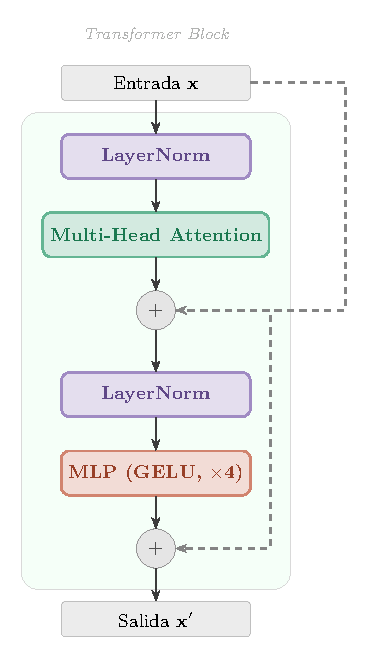
\includegraphics[width=0.40\textwidth]{images/diagrams_transformer/transformer_block.pdf}
    \caption{Bloque Transformer decoder-only (estilo GPT): Pre-LayerNorm seguida de Multi-Head Attention causal y MLP, con conexiones residuales. No incluye cross-attention ni componente recurrente; cada token solo atiende posiciones anteriores mediante causal masking.}
    \label{fig:block_transformer}
\end{figure}

% ---------------------------------------------------------------
\subsection{Token Embeddings y Positional Encoding}

Antes de entrar al primer bloque, cada token de la secuencia se convierte en un vector denso mediante una capa de embedding aprendible $E \in \mathbb{R}^{|V| \times d_{model}}$, donde $|V|$ es el tamaño del vocabulario. Para el token en posición $t$ con índice $w_t \in \{0, \ldots, |V|-1\}$:

\begin{equation}
    e_t = E[w_t] \in \mathbb{R}^{d_{model}}
\end{equation}

El modelo propuesto utiliza el vocabulario del tokenizador GPT-2 con $|V| = 50\,257$ y $d_{model} = 768$, resultando en una matriz de embedding de $50\,257 \times 768 = 38{,}6\text{M}$ parámetros. Para reducir el coste de memoria, los pesos de esta capa se comparten con la cabeza de predicción final (\textit{weight tying}): $W_{lm\_head} = E^\top$.

El mecanismo de atención es invariante a la permutación: procesa $\{e_1, \ldots, e_L\}$ sin noción de orden. Para dotar al modelo de información posicional, se añade un vector $p_t$ a cada embedding antes del primer bloque. La formulación sinusoidal de Vaswani et al.~\cite{vaswani2017attention} define:

\begin{equation}
    PE_{(t,\,2i)} = \sin\!\left(\frac{t}{10000^{2i/d_{model}}}\right), \quad
    PE_{(t,\,2i+1)} = \cos\!\left(\frac{t}{10000^{2i/d_{model}}}\right)
\end{equation}

donde $t$ es la posición del token y $2i$, $2i{+}1$ indexan las dimensiones del embedding por pares. Esta codificación es determinista y generaliza a longitudes no vistas durante el entrenamiento. El modelo propuesto utiliza embeddings posicionales \textit{aprendibles} (estilo GPT-2), donde $p_t$ es una fila de la matriz $P \in \mathbb{R}^{L_{max} \times d_{model}}$ optimizada junto con el resto de la red, ofreciendo mayor flexibilidad dentro del rango de contexto fijo $L \leq 1024$. La representación de entrada al primer bloque combina ambos vectores:

\begin{equation}
    x_t = e_t + p_t = E[w_t] + P[t]
\end{equation}

% ---------------------------------------------------------------
\subsection{Feed-Forward Network}

Cada bloque Transformer incluye, tras la capa de atención, una red de avance posición a posición (\textit{Feed-Forward Network}, FFN) aplicada de forma independiente a cada token:

\begin{equation}
    \text{FFN}(x) = \text{GELU}(x W_1 + b_1)\, W_2 + b_2
\end{equation}

donde $W_1 \in \mathbb{R}^{d_{model} \times d_{ff}}$ y $W_2 \in \mathbb{R}^{d_{ff} \times d_{model}}$. La dimensión interna $d_{ff} = 4 \cdot d_{model} = 3072$ actúa como espacio de proyección expandido donde el modelo puede representar combinaciones no lineales de las características extraídas por la atención. La función de activación GELU~\cite{hendrycks2016gelu} proporciona suavidad en el gradiente frente a ReLU, favoreciendo la convergencia en modelos de lenguaje. La FFN representa aproximadamente el 67\% del cómputo total por bloque.

% ---------------------------------------------------------------
\subsection{Layer Normalization y Conexiones Residuales}

La \textit{Layer Normalization}~\cite{ba2016layer} normaliza cada vector de activación individualmente sobre sus $d_{model}$ dimensiones:

\begin{equation}
    \text{LayerNorm}(x) = \frac{x - \mu}{\sqrt{\sigma^2 + \varepsilon}} \cdot \gamma + \beta
\end{equation}

donde $\mu$ y $\sigma^2$ son la media y varianza del vector $x \in \mathbb{R}^{d_{model}}$, $\varepsilon$ es una constante de estabilidad numérica, y $\gamma, \beta \in \mathbb{R}^{d_{model}}$ son parámetros aprendibles de escala y desplazamiento. A diferencia de Batch Normalization, opera sobre la dimensión de características de un único ejemplo, lo que la hace independiente del tamaño de batch y adecuada para secuencias de longitud variable.

El modelo propuesto adopta la variante \textbf{Pre-LayerNorm} (Pre-LN), donde la normalización se aplica antes de cada sublayer:

\begin{equation}
    x' = x + \text{Sublayer}(\text{LayerNorm}(x))
\end{equation}

frente al esquema Post-LN original de Vaswani et al., donde se aplica después. Pre-LN estabiliza el entrenamiento desde las primeras iteraciones al garantizar que los gradientes fluyen directamente a través de las conexiones residuales sin pasar por la normalización, reduciendo la sensibilidad al learning rate inicial.

% ---------------------------------------------------------------
\subsection{Causal Masking}

En un modelo decoder-only, cada token $t$ solo puede atender a posiciones anteriores $\{1, \ldots, t\}$ para preservar la propiedad autoregresiva. Esto se implementa mediante una máscara triangular inferior $M \in \{0, -\infty\}^{L \times L}$ aplicada sobre las puntuaciones de atención antes del softmax:

\begin{equation}
    M_{ij} = \begin{cases} 0 & \text{si } j \leq i \\ -\infty & \text{si } j > i \end{cases}
\end{equation}

\begin{equation}
    \text{Attention}(Q, K, V) = \text{softmax}\!\left(\frac{QK^\top + M}{\sqrt{d_k}}\right) V
\end{equation}

Los elementos con valor $-\infty$ colapsan a cero tras el softmax, anulando efectivamente la contribución de tokens futuros. Esta restricción convierte la MHA en \textit{MHA causal}, habilitando el entrenamiento por \textit{teacher forcing} con un único paso hacia adelante sobre toda la secuencia.

% ---------------------------------------------------------------
\subsection{Long Short-Term Memory (LSTM)}

Las \textit{Long Short-Term Memory}~\cite{hochreiter1997lstm}, propuestas por Hochreiter y Schmidhuber en 1997, introducen un mecanismo de memoria explícita mediante una \textbf{celda de estado} $c_t$ separada del estado oculto $h_t$. Dado un token de entrada $x_t$ y los estados anteriores $h_{t-1}$, $c_t$, la LSTM computa:

\begin{align}
    f_t &= \sigma(W_f x_t + U_f h_{t-1} + b_f) & \text{(puerta de olvido)} \\
    i_t &= \sigma(W_i x_t + U_i h_{t-1} + b_i) & \text{(puerta de entrada)} \\
    o_t &= \sigma(W_o x_t + U_o h_{t-1} + b_o) & \text{(puerta de salida)} \\
    \tilde{c}_t &= \tanh(W_c x_t + U_c h_{t-1} + b_c) & \text{(candidato de celda)} \\
    c_t &= f_t \odot c_{t-1} + i_t \odot \tilde{c}_t & \text{(estado de celda)} \\
    h_t &= o_t \odot \tanh(c_t) & \text{(estado oculto)}
\end{align}

donde $\sigma$ es la función sigmoide y $\odot$ el producto elemento a elemento. La \textbf{puerta de olvido} $f_t$ decide qué información descartar de la celda anterior; la \textbf{puerta de entrada} $i_t$ controla qué nuevo contenido escribir; la \textbf{puerta de salida} $o_t$ filtra qué parte del estado de celda se expone como $h_t$.

\begin{figure}[H]
    \centering
    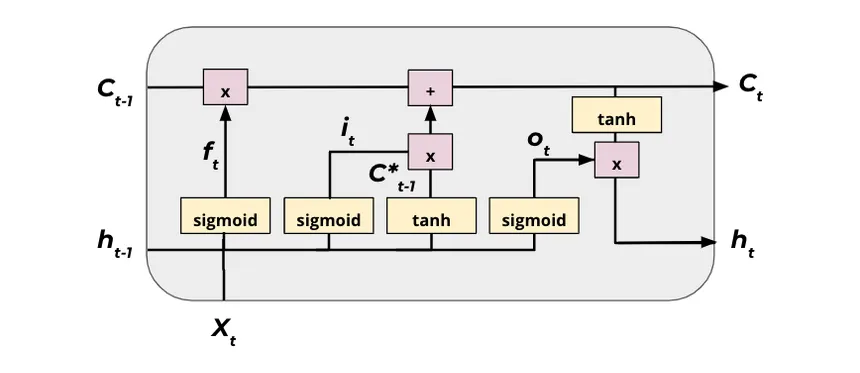
\includegraphics[width=0.72\textwidth]{images/fundamentos_teoricos/lstm_cell.png}
    \caption{Estructura interna de una celda LSTM. La celda de estado $c_t$ (línea superior) actúa como memoria a largo plazo controlada por tres puertas: olvido $f_t$ (rojo), entrada $i_t$ (verde) y salida $o_t$ (azul). El estado oculto $h_t$ es una proyección filtrada de $c_t$.}
    \label{fig:lstm_cell}
\end{figure}

% ---------------------------------------------------------------
\subsection{Gated Recurrent Units (GRU)}

Las \textit{Gated Recurrent Units}~\cite{cho2014learning} son una variante simplificada de las LSTM~\cite{hochreiter1997lstm} diseñada para reducir el número de puertas sin sacrificar capacidad de memoria selectiva. Dado un token de entrada $x_t$ y el estado oculto anterior $h_{t-1}$, el GRU computa:

\begin{align}
    z_t &= \sigma(W_z x_t + U_z h_{t-1} + b_z) & \text{(puerta de actualización)} \\
    r_t &= \sigma(W_r x_t + U_r h_{t-1} + b_r) & \text{(puerta de reinicio)} \\
    \tilde{h}_t &= \tanh(W_h x_t + U_h (r_t \odot h_{t-1}) + b_h) & \text{(candidato de estado)} \\
    h_t &= (1 - z_t) \odot h_{t-1} + z_t \odot \tilde{h}_t & \text{(estado oculto)}
\end{align}

donde $\sigma$ es la función sigmoide y $\odot$ denota el producto elemento a elemento. La \textbf{puerta de actualización} $z_t$ decide qué fracción del estado anterior se conserva; la \textbf{puerta de reinicio} $r_t$ controla cuánta información del pasado es relevante para computar el candidato $\tilde{h}_t$.

\begin{figure}[H]
    \centering
    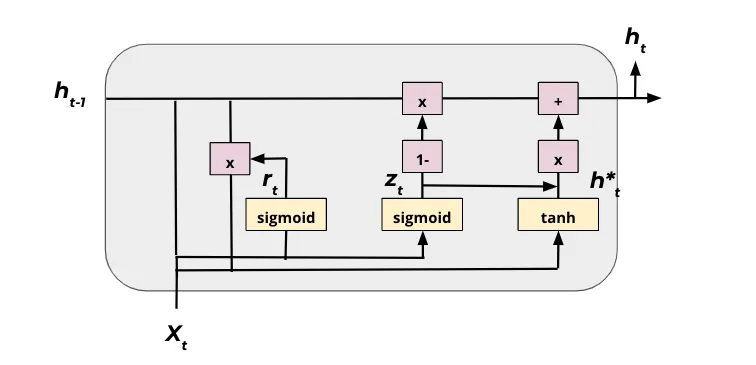
\includegraphics[width=0.72\textwidth]{images/fundamentos_teoricos/gru_cell.png}
    \caption{Estructura interna de una celda GRU. La puerta de reinicio $r_t$ (rojo) filtra cuánto del estado anterior $h_{t-1}$ se usa para calcular el candidato $\tilde{h}_t$ (verde). La puerta de actualización $z_t$ (morado) pondera la interpolación entre el estado anterior y el candidato para producir $h_t$.}
    \label{fig:gru_cell}
\end{figure}

\subsubsection{Justificación de GRU frente a LSTM}

La elección de GRU sobre LSTM está motivada por criterios de eficiencia en parámetros: una celda GRU tiene dos puertas frente a las tres de una LSTM (más la celda de memoria $c_t$), lo que reduce el número de parámetros por unidad en aproximadamente un 25\%. Estudios empíricos como los de Chung et al.~\cite{chung2014empirical} demuestran que esta reducción no implica pérdida significativa de rendimiento en tareas de modelado del lenguaje cuando el estado oculto tiene dimensión suficiente. En el contexto de un SLM con recursos limitados, esta eficiencia es determinante.

% ---------------------------------------------------------------
\subsection{La Hipótesis Híbrida: Análisis de Complejidad}

La motivación central de este trabajo es la superación del paradigma de \textit{``atención pura''} para modelos de escala reducida. La arquitectura híbrida propuesta se fundamenta en un análisis de complejidad comparativo entre los tres enfoques posibles:

\begin{table}[H]
\centering
\begin{tabularx}{\textwidth}{|X|c|c|c|}
\hline
\textbf{Arquitectura} & \textbf{Memoria} & \textbf{Cómputo} & \textbf{Estado secuencial} \\ \hline
Transformer puro & $O(L^2)$ & $O(L^2 d)$ & KV Cache (crece con $L$) \\ \hline
RNN / GRU puro & $O(d)$ & $O(Ld^2)$ & Estado fijo $h \in \mathbb{R}^d$ \\ \hline
\textbf{Híbrido (propuesto)} & $O(L^2 + d)$ & $O(L^2 d + Ld^2)$ & KV Cache + estado GRU \\ \hline
\end{tabularx}
\caption{Comparativa de complejidad computacional y de memoria.}
\label{tab:complejidad}
\end{table}

El diseño híbrido no mejora la complejidad asintótica en el peor caso, pero ofrece ventajas prácticas relevantes para el rango de contextos cortos-medios ($L \leq 1024$) en los que opera este modelo:

\begin{enumerate}
    \item \textbf{Eficiencia de memoria por bloque:} el GRU actúa como un \textit{compresor de contexto}, manteniendo un estado interno fijo $h \in \mathbb{R}^d$ que resume el historial de la secuencia sin necesidad de almacenar las activaciones intermedias de todos los tokens anteriores.
    \item \textbf{Separación de responsabilidades:} la atención captura dependencias globales de largo alcance, mientras el GRU modela la estructura secuencial local (orden de palabras, concordancia morfológica). Esta división evita que un único mecanismo deba resolver ambas escalas, reduciendo la carga efectiva de cada componente.
    \item \textbf{Inferencia estable en contextos largos:} el estado oculto del GRU permanece acotado independientemente de $L$, proporcionando una representación del historial con latencia constante que complementa el KV Cache de atención.
\end{enumerate}